Dans le cadre de la réponse à l’appel à projet pour le plan triennal de la recherche de la \indexmot{Bibliothèque nationale de France}, le programme \enquote{La couleur~: artefacts, matière et cognition} prévoit tout un volet d'éditorialisation à partir des données récoltées et analysées. L'éditorialisation doit permettre de \enquote{«répondre aux différents besoins des communautés scientifiques travaillant sur la couleur et ses matériaux\footnote{Appel à projet « La couleur~: artefacts, matière et cognition »}}. Les données sont, pour leur part, renseignées dans une base qui est développée et hébergée par l’Institut national d’histoire de l’art (INHA). La base repose sur un modèle structuré : les données sont hiérarchisées et suivent des référentiels spécialisés. Le programme de recherche \enquote{La couleur : artefacts, matière et cognition} est également lié au programme de recherche de Sigrid Mirabaud sur \enquote{La fabrique matérielle du visuel~: panneaux peints en Méditerranée, XIIIe-XVIe siècle}. Les \indexmot{visualisation}s envisagées et évoquées au cours de ce mémoire concernent les deux projets. \par
Ce chapitre revient sur les étapes qui précèdent et qui permettent l’éditorialisation des données. Il s’agit, d’une certaine façon, d’un chapitre préliminaire à la présentation du travail réalisé au cours de ce stage. Cependant, les pages qui suivent permettent de comprendre les chemins que pouvaient prendre le travail de \indexmot{visualisation} à partir des données présentes. \newpage

\section{Les bases de donnée}

Les programmes de recherche sur \enquote{La couleur : artefacts, matière et cognition} et sur \enquote{La fabrique matérielle du visuel~: panneaux peints en Méditerranée} débutent en janvier 2021. Les premiers temps du projet sont consacrés à la constitution d’un corpus d’œuvres à soumettre aux analyses. Il s’agit principalement de collections du département des manuscrits pour le premier projet. Un peu plus de trois années après le lancement, en juin 2024, trois cent trente-six manuscrits et panneaux peints en ont fait l’objet. Le résultat est un ensemble de données, issues de rapports d’analyses physico-chimiques. Elles proviennent de différents laboratoires avec lesquels la \indexmot{Bibliothèque nationale de France} a conclu des accords~: le Centre de Recherche et de Restauration des Musées de France (C2RMF), l’Institut de recherche sur les archéomatériaux Centre Ernest-Babelon (IRAMAT-CEB), le laboratoire de recherche des monuments historiques (LRMH) ou encore le Centre de Recherche sur la Conservation (CRC). Depuis le début du projet, un carnet de recherche accompagne les travaux menés et leur assure une publicité et une diffusion auprès du public (https://couleur.hypotheses.org). Ce carnet permet également de refléter les croisements interdisciplinaires qui entourent le projet~: histoire de l’art, histoire, archéologie, linguistique, anthropologie, mais aussi, nous l’avons vu, des disciplines issues des sciences dites « dures ». La réunion de chercheurs de traditions scientifiques différentes a produit de nouveaux \indexmot{thésaurus} qui viennent enrichir la description des enluminures, que ce soit pour les matériaux ou les techniques. Aujourd’hui, le projet est à sa phase finale~: les dernières données collectées sont intégrées dans Agorha et la migration vers deux sites Omeka S est prévue pour l’automne. Les \indexmot{visualisation}s réalisées dans le cadre de ce stage trouveront place sur ces derniers. \newline\par
La base produite à l’issue des programmes de recherche contient des données de différentes natures sur les manuscrits et les panneaux peints.
\begin{enumerate}
	\item Premièrement, elle contient des informations propres à chaque objet du corpus~: l’identifiant, la cote ou l’inventaire, l’auteur, la date, l’origine ou encore les dimensions. Ces informations permettent d’identifier l’objet dont il est question, de le recenser au sein du corpus et de le situer pour le public. Ces métadonnées sont le point de départ des interprétations qui sont réalisées avec le résultat des analyses. Elles attachent ces dernières à un contexte et à un cadre de production auxquels il faut toujours se référer.
	\item Ensuite, chaque entrée de la base de données est reliée à une image numérique. Cette image est une reproduction de l’objet analysé. Elle a une double utilité. Elle permet, dans un premier temps, à l’utilisateur de prendre connaissance de l’enluminure avec les métadonnées précédemment décrites. Ensuite, l’image numérique change de sens pour devenir un outil, pour un regard plus précis sur les zones analysées et renseignées dans le point suivant.
	\item En troisième lieu, la base contient toutes les analyses physico-chimiques et techniques réalisées au cours des deux projets de recherche. Ces données renseignent sur la localisation des analyses, avant de passer à la présentation des matériaux pour les couleurs observées~: pigments, colorants, liants, vernis. Les données sont interprétées, datées et sourcées. Elles sont issues des \indexmot{thésaurus} réalisés et sont ainsi normalisées.
	\item Enfin, la base fournit une documentation complémentaire relative à la conservation et à la restauration, une bibliographie spécialisée sur les matériaux, des liens vers les manuscrits numérisés (Gallica) ou encore vers des corpus de sources textuelles sur les pigments (recettes médiévales, traités théoriques…).
\end{enumerate} \par
Le travail d’éditorialisation des données des bases est réalisé à partir de fichiers CSV. Cependant, les données sont visibles pour le public sur le site Agorha pour le moment, puis sur les sites Omeka S à l’automne 2024. Cette exploration des données par une navigation internet fait partie prenante des projets et conditionne, aussi, les \indexmot{visualisation}s qui seront produites. \newpage

\section{La plateforme Agorha}

Mise en ligne en 2011, refondée en 2021, Agorha a aujourd’hui plus de 250 000 notices sur son site. Il donne un accès aux bases de données produites par l’INHA et ses partenaires, comme le département des manuscrits dans le cas présent. Ces données sont issues de programmes de recherche scientifique en histoire de l’art et archéologie. Agorha n’a pas donc pas vocation à l’exhaustivité, mais à proposer une sorte de bibliothèque numérique choisie à ses utilisateurs. Une bibliothèque de référence, qui témoigne d’une recherche numérique ouverte, d’une science partagée. \par
Les données produites sont organisées selon des notices décrivant des œuvres, des personnes et organismes, des références bibliographiques et d’archives, des collections et des événements. Ces notices sont enrichies collaborativement. La plateforme est pensée pour que les notices puissent être liées entre elles, indépendamment de leur type ou des programmes de recherche auxquels elles sont rattachées ; une même notice peut être ainsi reliée à différents programme de recherche. Les données sont également constituées de médias. Elles enrichissent les notices avec des fichiers, principalement d’images. Outre les liens faits entre les notices, celles-ci peuvent aussi être liées à des \indexmot{thésaurus} et ainsi renvoyer à des référentiels de vocabulaire interne ou externe de l’INHA. Je reviendrai sur la question des termes contrôlés plus en avant. \newline\par
Le 1er juillet 2024, Agorha compte 1136 notices pour le projet sur la couleur du département des manuscrits. Toutes ne sont pas encore publiées et disponibles en ligne à cette date, mais elles le seront d’ici l’automne. Ces notices sont majoritairement des œuvres (1013), mais elles portent aussi sur des références (93), des personnes (28) et des collections (2). Il n’y a pas de notice sur des événements. Le projet sur les panneaux a, à la même date, 762 notices~: 227 œuvres, 5 personnes et 530 références.\par
La structuration d’une notice Agorha tient en deux temps pour l’utilisateur. Le premier est celui où il la découvre par son média – ici son image – et les liens qu’elle peut entretenir avec d’autres notices. Il s’agit d’un premier carrousel d’images. En bas de la page, une second carrousel permet d’afficher toutes les œuvres, toutes les personnes ou encore toutes les références liées à la notice en cours. \textit{Voir la figure~1.} \par

\begin{figure}[p]
	\centering
	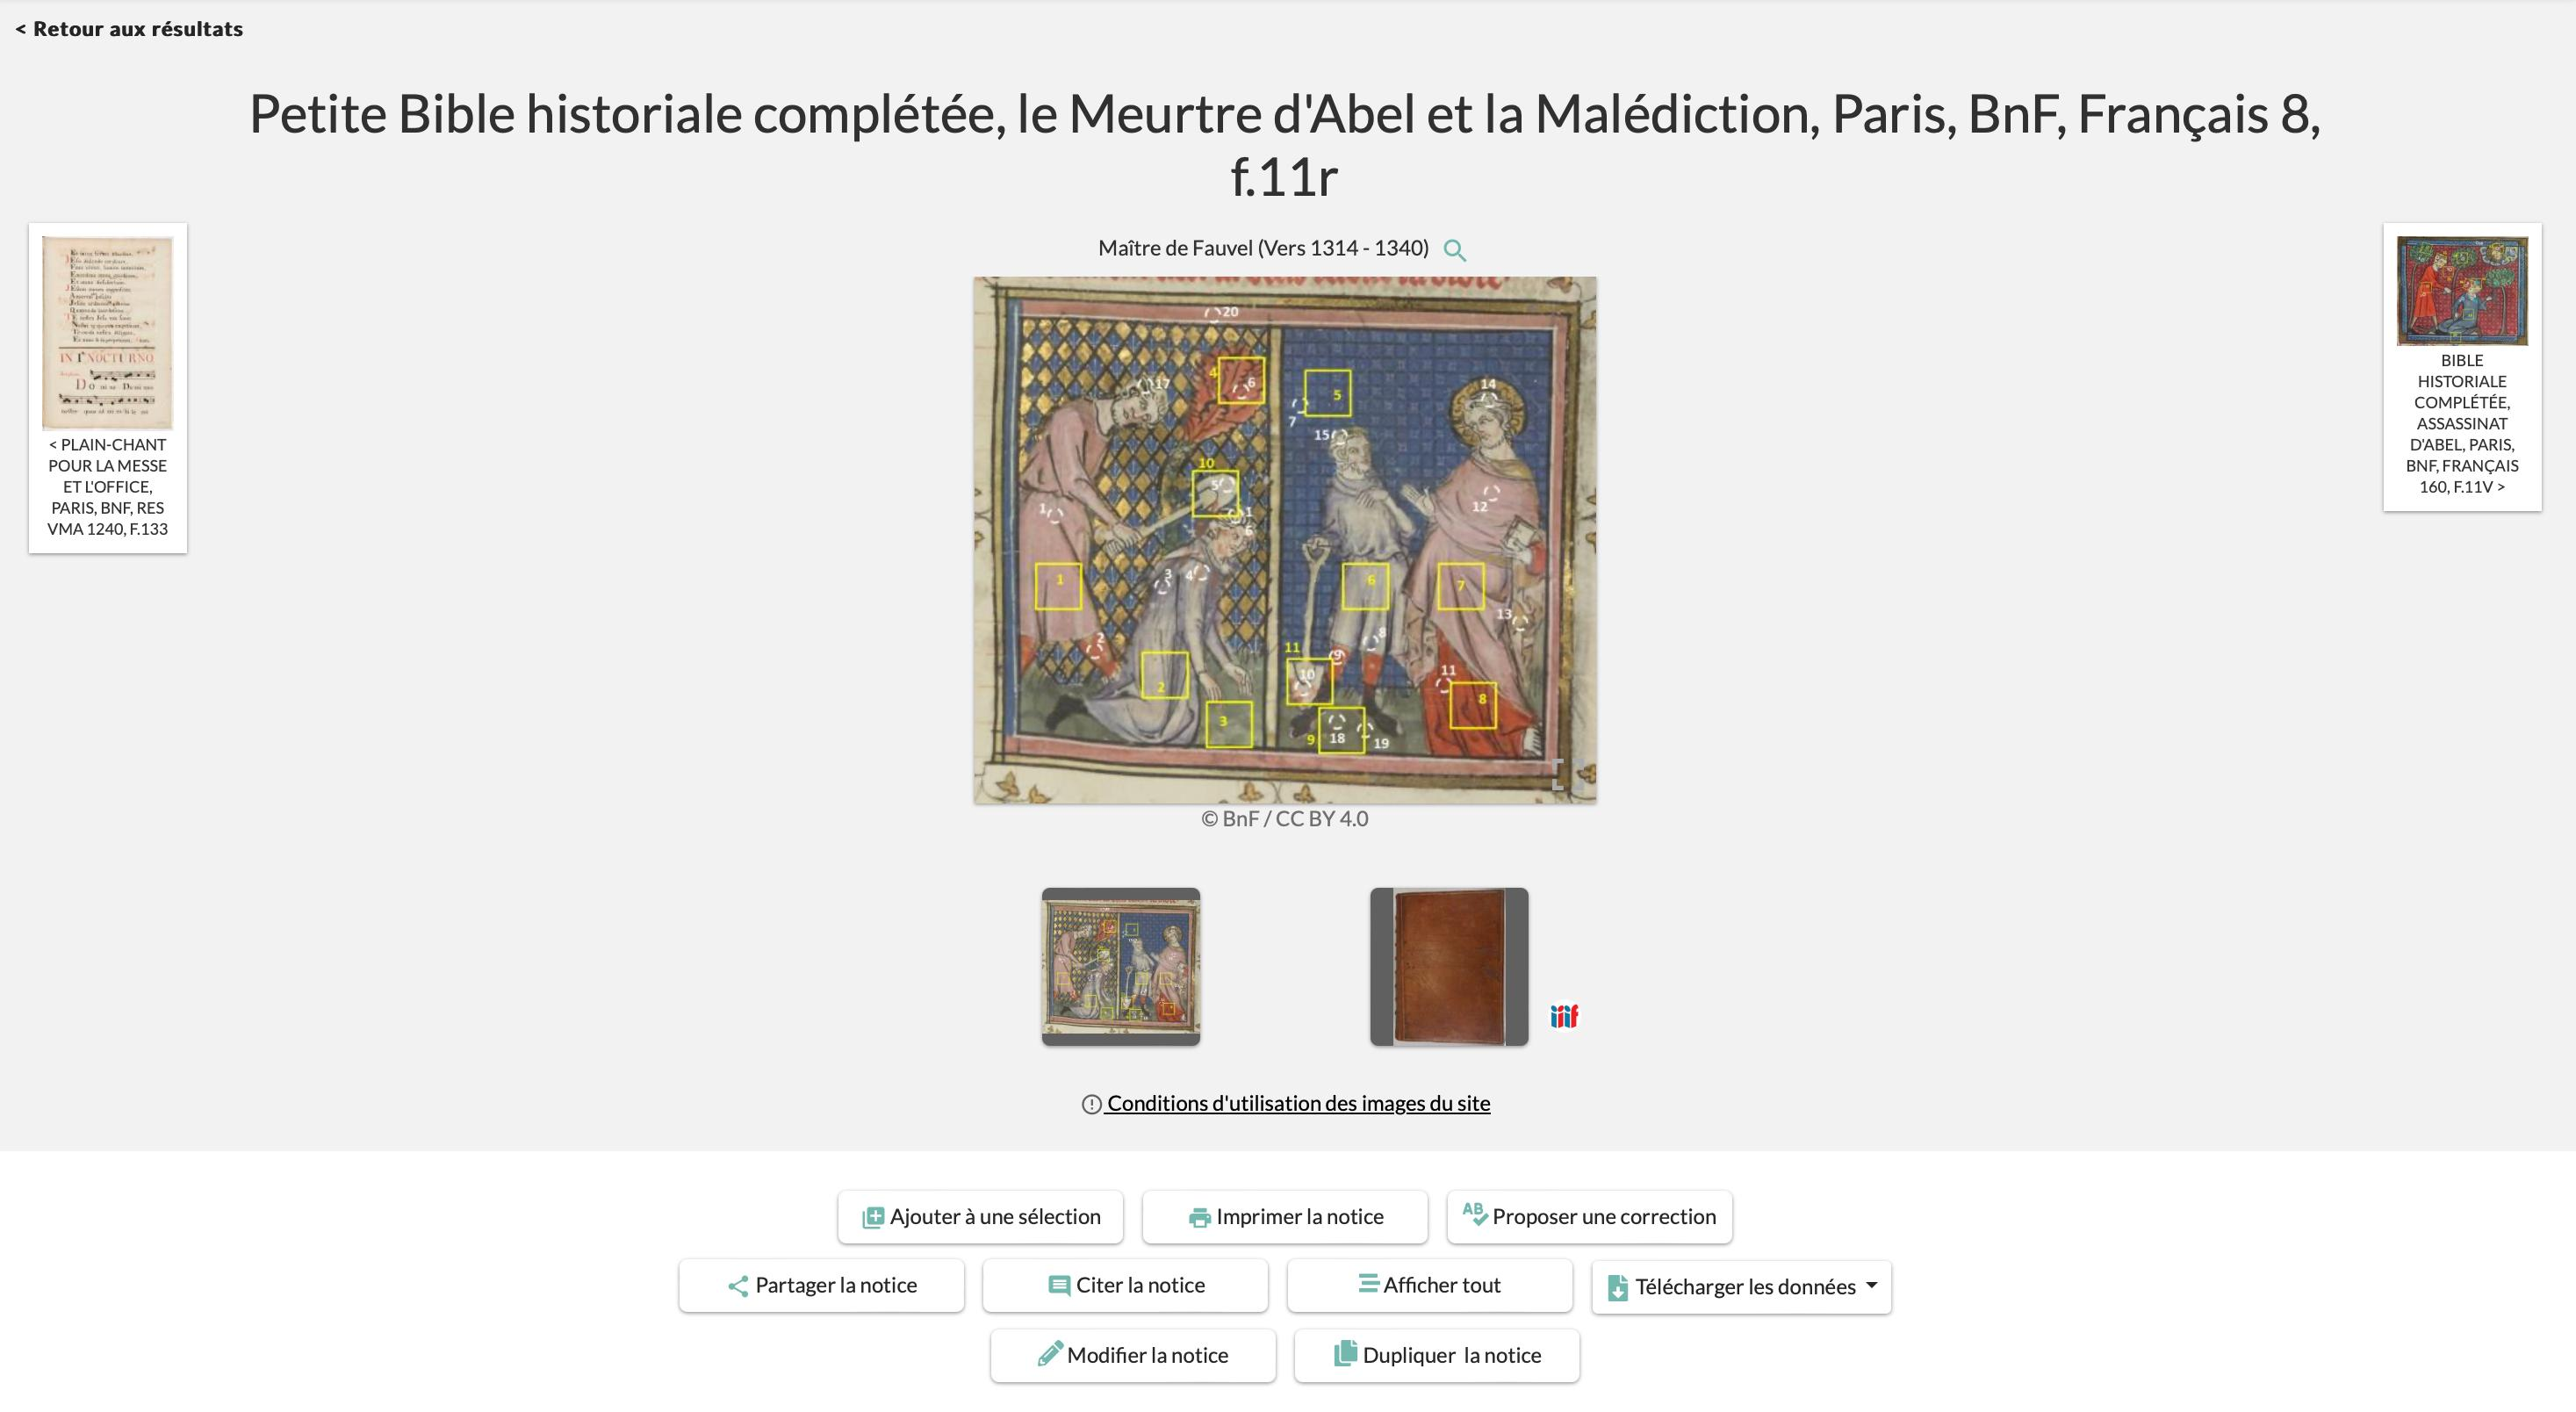
\includegraphics[width=\textwidth]{./textes/chap1/agorha-carrousel.jpg}
	\caption{Le média d'une notice Aghora}
	\label{fig:carrousel}
\end{figure}

Ensuite, la notice repose sur des champs de données structurées. Les informations sur les feuillets des manuscrits sont divisées entre plusieurs catégories, selon le besoin des projets. Pour le projet sur la couleur, huit champs de données sont retenus : l’identification, la localisation, la description (avec les analyses), la création, la qualification entre l’imprimé et le manuscrit, les liens entre les œuvres, la documentation et, pour finir, la gestion de la notice. Ces champs sont à leur tour divisés en de nouveaux qui contiennent les résultats des projets de recherche, soit sous la forme d’une entrée de \indexmot{thésaurus}, soit d’un texte libre entré par la personne qui saisit. \textit{Voir la figure~2.}\par

\begin{figure}[p]
	\centering
	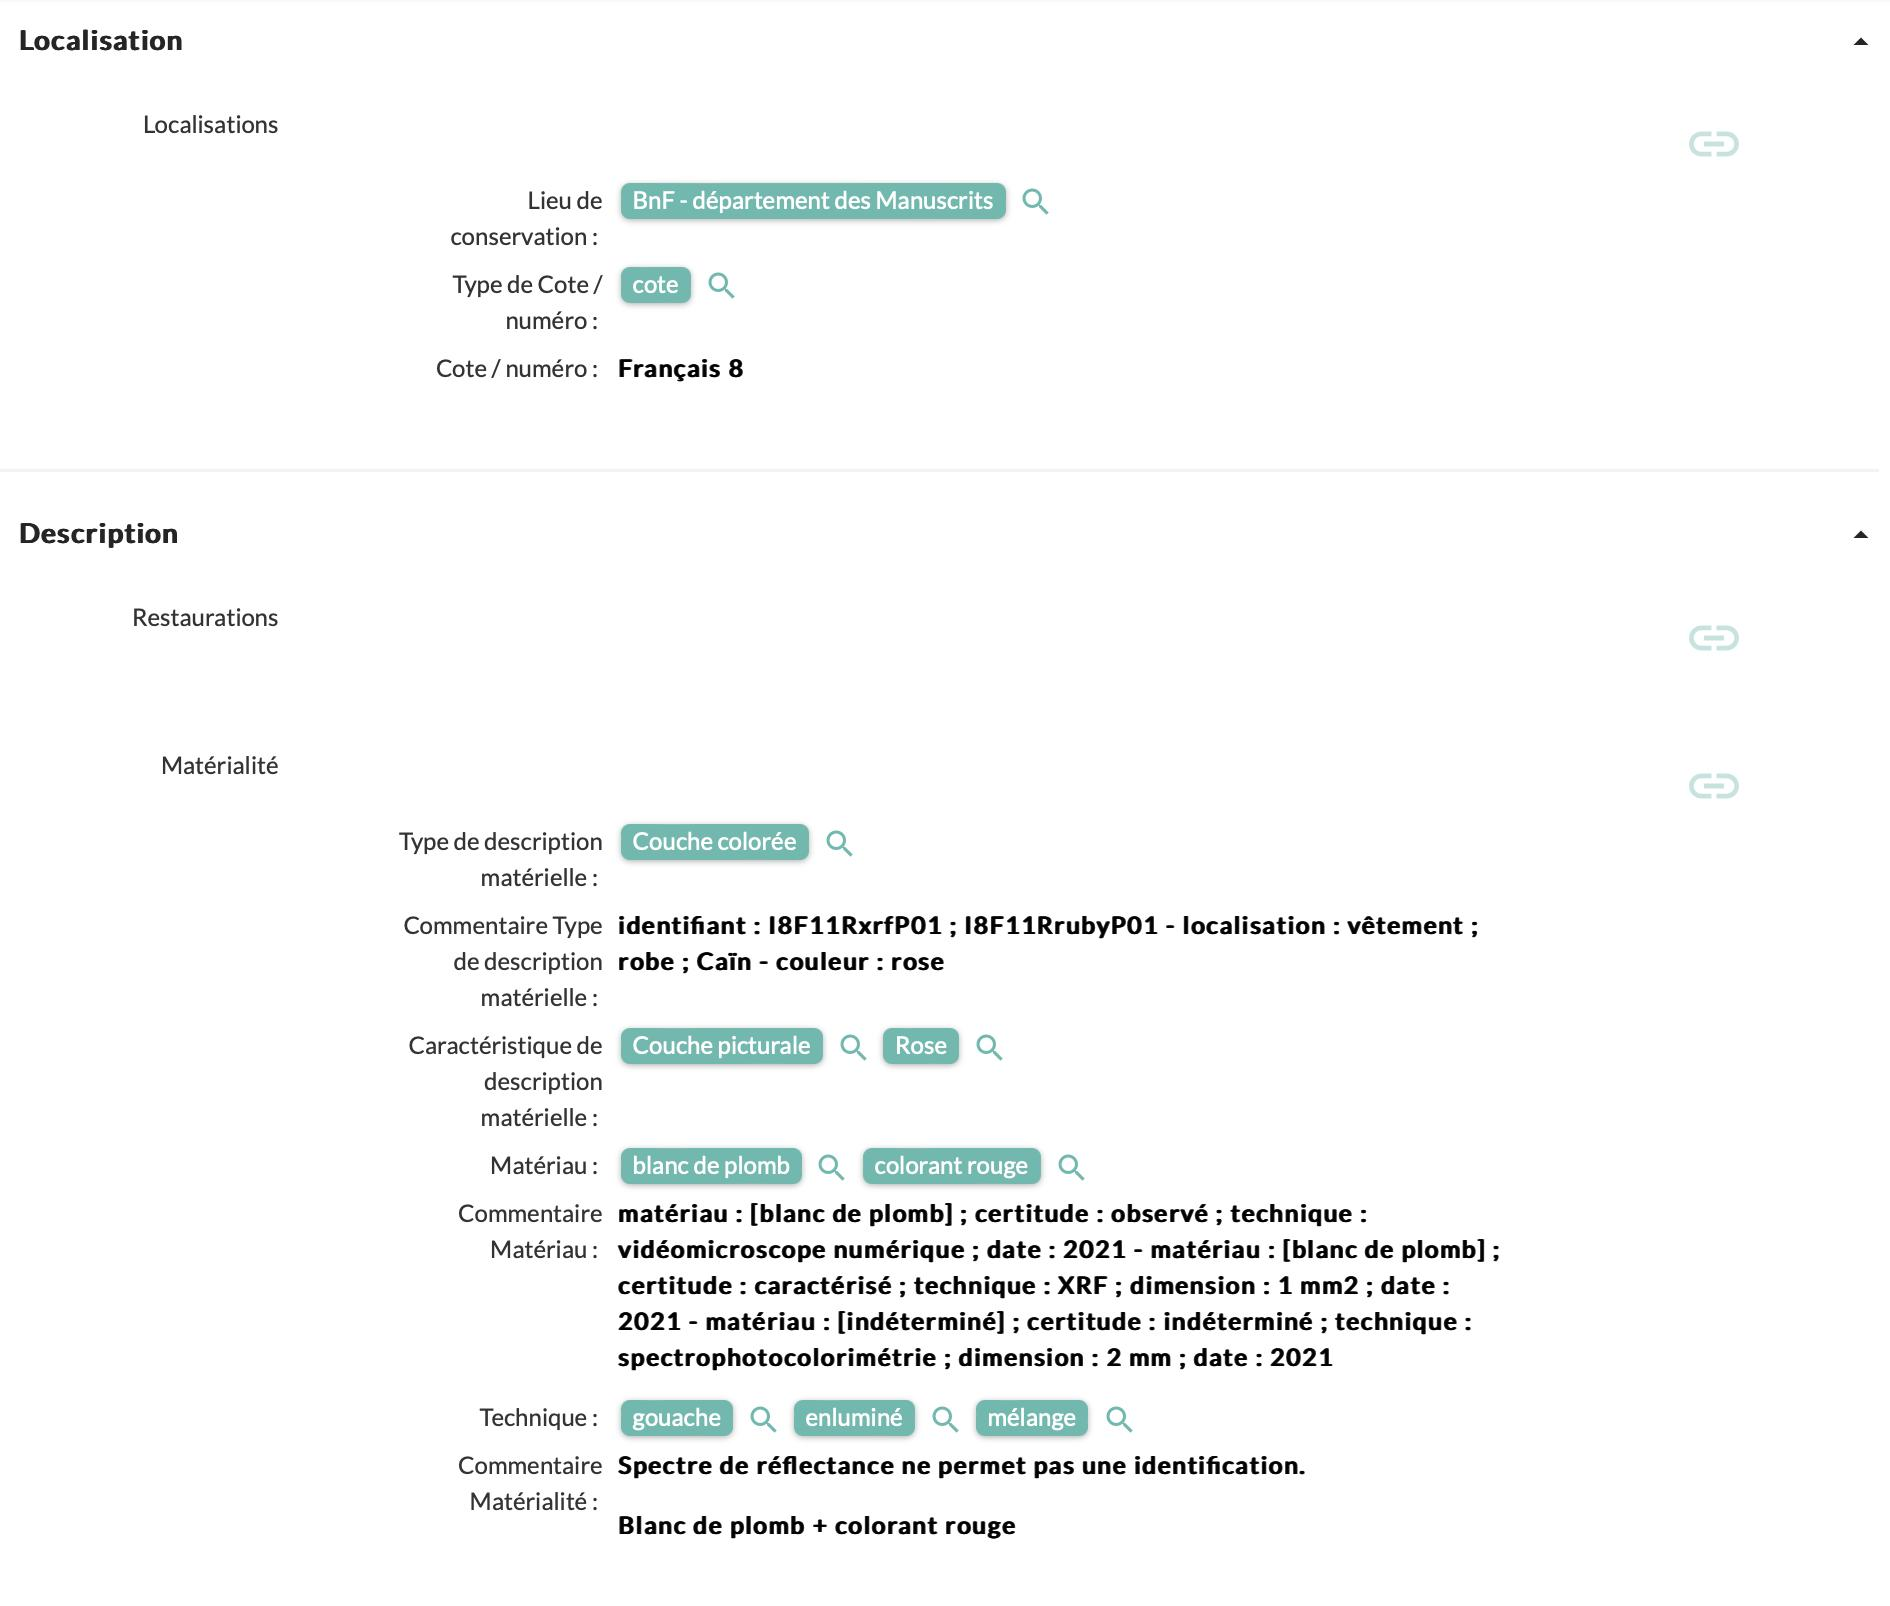
\includegraphics[width=\textwidth]{./textes/chap1/agorha-info.jpg}
	\caption{Les champs structurés sur Agorha}
	\label{fig:info}
\end{figure}

Les notices ont des identifiants uniques attribués automatiquement par le système informatique d’Agorha. L’identifiant est présent dans l’URL, c’est un UUID (Universally unique identifier). Pour retrouver une notice, il suffit ainsi de le renseigner à la fin de l’adresse d’Agorha~: \par
https://agorha.inha.fr/ark:/54721/ + UUID \\\par
En anticipant un peu sur la suite de ce mémoire, il convient ici de souligner que les notices œuvres concernent des feuillets de manuscrit. À titre d’exemple, le verso du feuillet~91 du manuscrit syriaque~47 a pour adresse https://agorha.inha.fr/ark:/54721/4308c58d-6569-489e-8d7d-a7436872b5cd?database=89. Son identifiant est donc~: 4308c58d-6569-489e-8d7d-a7436872b5cd. Ce système d’identification unique, avec le même nombre de caractères, facilite la récupération d’informations et la structuration des différentes notices entre elles, nous le verrons plus en avant. \par
Pour revenir à Agorha, ces identifiants uniformes permettent à la plateforme de s’insérer pleinement dans le web de données liées\footcite{pochon_agorha_nodate}. Ce dernier repose sur un ensemble de bonnes pratiques pour publier et relier des données structurées sur le web. Il vise principalement à faciliter l'intégration et l'interconnexion de données provenant de diverses sources. Agorha suit le modèle RDF (Resource Description Framework) qui représente les informations sous forme de triplet : un sujet, un prédicat, un objet. Par exemple, un feuillet (sujet) est réalisé à (prédicat) tel endroit (objet). La multiplication de triplets RDF permet de constituer un ensemble qui structure et interconnecte les informations. Les données liées peuvent ensuite être sérialisées avec du JSON-LD. Cette syntaxe permet de représenter des graphes RDF de manière compacte et facile à intégrer dans des applications web, tout en conservant les capacités de lien et de description du RDF. Dans Agorha, toutes les notices reposent sur du JSON-LD. Pour faire apparaître la méthode, il suffit de compléter les adresses de cette façon~:\par https://agorha.inha.fr/ark:/54721/ + UUID + .json. \newline\par
Si nous nous penchons sur le cas du manuscrit syriaque précédent, sa localisation apparaît ainsi en JSON-LD~:

\begin{lstlisting}[language=json]
"localizationInformation" : {
	"localization" : [ {
		"place" : {
			"thesaurus" : {
				"ref" : "https://thesaurus.inha.fr/thesaurus/resource/ark:/54721/bd1b5af3-9b44-49e9-98b8-b97ca10dd7f2",
				"prefLabels" : [ {
					"value" : "\indexmot{Bibliothèque nationale de France} (Paris)",
					"language" : "fre"
				} ],
				"conceptPath" : "/Europe/France/Ile-de-France/Paris/\indexmot{Bibliothèque nationale de France} (Paris)",
				"geoPoint" : "48.834355,2.373378"
			}
		},
		"institutionIdentifierType" : {
			"thesaurus" : {
				"ref" : "https://thesaurus.inha.fr/thesaurus/resource/ark:/54721/feccfc54-f2da-458a-a42c-530037a5132b",
				"prefLabels" : [ {
					"value" : "cote",
					"language" : "fre"
				} ],
				"conceptPath" : "/cote"
			}
		},
		"institutionIdentifier" : {
			"value" : "Syriaque 47",
			"language" : "fre"
		},
		"sourcing" : [ {
			"database" : {
				"ref" : "89",
				"value" : "La fabrique de l'art. Couleurs et matériaux de l'enluminure"
			}
		} ]
	} ]
}
\end{lstlisting} \par
Agorha permet donc une intégration structurée et interconnectée des résultats des deux programmes de recherche sur le web. La plateforme de l’INHA contribue à la science ouverte et la communication des résultats des analyses sur les enluminures et les panneaux peints selon les principes du web de données liées. \newpage

\section{Deux sites Omeka~S}

Les deux projets ne seront pas seulement présents sur la plateforme Agorha. L’INHA développe en ce moment deux sites Omeka~S qui permettront d’héberger, à partir de l’automne, les bases de données ainsi que les \indexmot{visualisation}s réalisées. Cette plateforme open source est spécifiquement conçue pour gérer des collections numériques dans l’optique d’une publication en ligne\footcite{noauthor_omeka_nodate}. Elle semble parfaitement correspondre aux attentes d’un projet de recherche scientifique comme ceux sur les manuscrits ou les panneaux peints.\par
En premier lieu, le site Omeka~S permet de créer des collections numériques. Ces dernières peuvent contenir les différentes notices présentes sur Agorha, mais avec une organisation et un archivage qui sont facilités. De plus, l’utilisation du schéma de métadonnées Dublin Core permet de reprendre les éléments des descriptions détaillées des notices. Il n’y a pas de perte de l’information et la normalisation reste. Ensuite, Omeka~S est conçu pour intégrer les données RDF que j’ai présentées précédemment. L’interconnexion entre les différentes données des résultats existera toujours. Il en est de même avec le JSON-LD. Omeka~S permet aussi d'accéder et de manipuler les données via des API, ce qui correspond aussi au critère d’interopérabilité voulu. Le principal avantage, au regard de la plateforme Agorha, réside dans la possibilité de le personnaliser pour les besoins spécifiques du projet. Le site public peut être structuré pour correspondre le mieux possible aux deux bases : navigation entre les onglets, liens entre les pages, visibilité des résultats ou encore insertion des \indexmot{visualisation}s. Le module de recherche lui-même peut être amélioré, afin d’orienter l’utilisateur vers des filtrages, option indispensable pour les projets scientifiques aussi complexes. Avec le site Omeka~S, les utilisateurs pourront sélectionner des paramètres parfois très précis pour isoler certains résultats ou croiser plusieurs filtres afin de faire apparaître des correspondances. En dernier lieu, un site conçu sur Omeka~S est traditionnellement conforme aux standards archivistiques et de gestion des collections, garantissant la pérennité des données. En outre, sa conception est conforme aux normes d’accessibilité, rendant le site utilisable par toute sorte de public.\par
En ce qui concerne les trois \indexmot{visualisation}s proposées pour les projets de recherche, leur intégration dans Omeka~S varie. L’intégration par iframe semble être la meilleure solution pour ce qui est de la \indexmot{carte interactive} et de la \indexmot{frise chronologique}. Un iframe, c’est~:\par
\begin{quote}
	« un élément HTML qui permet d'intégrer un contenu externe dans une page web. L'Iframe peut contenir une vidéo, une carte, une publication de réseau social ou encore une page web tierce. Le contenu s'affiche dans un cadre dont les propriétés peuvent être paramétrées à l'aide d'attributs.\footcite{thach_quest-ce_nodate} »
\end{quote}\par
En récupérant le contenu des deux \indexmot{visualisation}s et en personnalisant leur affichage, le site Omeka~S devrait permettre une navigation confortable pour l’utilisateur. Pour ce qui est des manifestes \indexmot{IIIF} et de leur exploration dans une visionneuse, il ne pouvait être raisonnablement proposé de passer par la solution d’un Iframe. En effet, Omeka~S permet d’implémenter directement une visionneuse, comme Mirador, dans le site réalisé. Cependant, la visionneuse étant insérée par un module propre à Omeka, elle ne possède pas les mêmes propriétés que celle en libre accès sur internet. Un problème de compatibilité des manifestes \indexmot{IIIF} est apparu alors, j’y reviendrai plus un avant.\newpage

\section{L’enjeu du \indexmot{thésaurus}}

Les \indexmot{visualisation}s sont, dans le fond, une certaine forme d’éditorialisation de la donnée. Elles reposent sur une interrogation des jeux et des entrées présents dans la base. Ainsi, plus les termes et les catégories utilisés lors de sa conception sont précis et cohérents, plus la \indexmot{visualisation} sera pertinente d’un point de vue scientifique au moment de sa réalisation. Il me semble que la constitution des \indexmot{thésaurus} a joué un rôle déterminant dans la réussite des deux projets et a permis d’envisager les différentes \indexmot{visualisation}s. Je souhaite donc m’y attarder un moment pour finir ce chapitre introductif. \par
Un \indexmot{thésaurus} est, en quelque sorte, une standardisation du vocabulaire. Son rôle est de garantir que les termes sont utilisés de manière uniforme tout au long du travail de recherche. C’est un vocabulaire contrôlé, qui doit prévenir les éventuelles ambiguïtés et incohérences dans le remplissage des données dans la base. Mais au-delà de cette normalisation, l’instauration d’un \indexmot{thésaurus} est fondamentale en ce qu’il contraint les chercheurs à une réflexion sur les termes utilisés et leur articulation les uns avec les autres. Ainsi, le \indexmot{thésaurus} aide à structurer la description. L’attribution d’un terme à une donnée, à une idée, à une réalité – ce qui est donc une indexation – peut induire une hiérarchie en fonction du vocabulaire retenu. Les données sont alors regroupées selon leur similarité et classées par une logique définie en amont. Ce vocabulaire nécessite un effort théorique de la part des coordinateurs du projet~: les termes doivent être justifiés et explicités et, bien souvent, une documentation est produite pour accompagner un \indexmot{thésaurus}. Elle permet de fournir des définitions claires et précises des termes, des orientations aussi quant à l’indexation à choisir. \\\par
Les porteurs du projet ne cachent pas que l’un des principaux défis a bien été la constitution d’un référentiel d’autorité sur les matériaux et les couleurs qui puisse être applicable à des techniques, des époques et des aires géographiques très diverses\footnote{Appel à projet « La couleur~: artefacts, matière et cognition »}. S’il existait déjà un \indexmot{thésaurus} de référence pour les sciences de la conservation\footnote{Vocabulaire contrôlé réalisé pour les projet PARCOURS, puis SOCORÉ.}, ce n’était pas le cas pour la couleur et ses composants. Quelques précédents étrangers peuvent servir d’exemples cependant, comme la base américaine CAMEO\footcite{conservation__art_materials_encyclopedia_online_pigment_nodate}. L’élaboration du référentiel des matières colorantes est un parfait exemple de la synergie entre les différentes traditions scientifiques qui entourent le projet, puisqu’elle est le fruit d’ateliers réunissant des spécialistes de diverses disciplines (historiens de l’art, chimistes, spécialistes des textes anciens, naturalistes, anthropologues, etc.) et des professionnels issus des institutions partenaires. 
Une fois créés, les \indexmot{thésaurus} « matériaux » et « techniques » viennent enrichir GINCO (Gestion d’Informations Communes). GINCO donne accès à l’ensemble des vocabulaires scientifiques et techniques produits par le Ministère de la Culture et ses partenaires\footcite[En 2024, le logiciel n’est plus maintenu à jour et semble voué à disparaître.]{ministere_charge_de_la_culture_culturecommunicationginco_2022}. L’INHA, pour ses projets, se fournit et alimente les vocabulaires établis, au  moyen du langage de requête SPARQL\footcite{inha_thesaurus_nodate}. De façon concrète, dans le cadre des deux projets qui nous intéressent, le chercheur qui saisit des données dans la base le fait par l’intermédiaire de champs de recherche. À ce moment, un petit moteur de recherche suggère par auto-complétion les termes qui pourraient convenir et qui sont présents dans GINCO. Si aucun terme ne convient, il faut que le chercheur demande son ajout dans le \indexmot{thésaurus}, le vocabulaire serait alors renseigné au format SKOS\footcite[« SKOS (Simple Knowledge Organisation System ou Système simple d’organisation des connaissances) est un langage de représentation de schémas de concepts, ce qui recouvre les langages documentaires tels que les \indexmot{thésaurus}, classifications, listes de vedettes matière, taxonomies, folksonomies, etc. Son nom a été choisi pour mettre en évidence l’objectif même visé par ce langage : proposer un système permettant d’exprimer et de gérer des modèles interprétables par les machines dans la perspective du web sémantique », ][]{lenart_skos_2007} pour pouvoir intégrer GINCO. Cette méthode de travail et de complétion de la base permet de s’assurer de la cohérence du vocabulaire utilisé et de sa normalisation.

Concernant les \indexmot{visualisation}s des jeux de données, la constitution d’un \indexmot{thésaurus} commun aux deux projets permet de les réunir au sein d’un même travail d’éditorialisation. L’utilisation d’un vocabulaire contrôlé identique, pour la recherche sur \enquote{La couleur~: artefacts, matière et cognition} et sur \enquote{La fabrique matérielle du visuel~: panneaux peints en Méditerranée}, autorise leur interrogation selon les mêmes critères et pour l’ensemble des résultats. Cette démarche simplifie aussi le travail technique qui poursuit les projets. La définition des filtres, qui sont les pivots de l’éditorialisation, ne représente dès lors plus un enjeu puisqu’ils sont communs et choisis par les chercheurs. Il n’y aura ni ambiguïté, ni incohérence. \newpage

* \\

Depuis le début du projet, en janvier 2021, les différents porteurs ont œuvré pour que les données constituées dans la base s’inscrivent dans les nouvelles recommandations de l’interopérabilité et dans une politique de science ouverte. La communication des résultats avec le public des chercheurs est pensée en deux temps~: une première sur la plateforme Agorha de l’INHA, où les données rejoignent~–~et sont valorisées avec~–~d’autres programmes de recherche en histoire de l’art et archéologie~; et une seconde, avec une migration des données vers deux sites Omeka~S, afin d’individualiser et de personnaliser les résultats du projet. La constitution de \indexmot{thésaurus} identiques aux deux recherches permet de proposer des \indexmot{visualisation}s communes et ainsi de poursuivre leur collaboration.